\documentclass[11pt, a4paper]{article}
\usepackage{graphicx}
\usepackage{amsmath}
\usepackage{listings}
\usepackage{mathrsfs}



\title{Assignment 8} % Title

\author{Om Shri Prasath (EE17B113)} % Author name

\date{\today} % Date for the report
\begin{document}	

\maketitle % Insert the title, author and date
\section{Introduction}\label{introduction}

\begin{itemize}

\item
  We analyse and use DFT to find the Fourier transform of
  periodic signals and non periodic ones using fast fourier transform
  algorithms which are implemented in python using \(fft\) and
  \(fftshift\) which is used to center the fourier spectra of a discrete
  signal.
\item
  The discrete Fourier transform (DFT) converts a finite sequence of
  equally-spaced samples of a function into a same-length sequence of
  equally-spaced samples of the discrete-time Fourier transform (DTFT),
  which is a complex-valued function of frequency.
\item
  Let suppose f{[}n{]} are the samples of some continous function
  \(f(t)\) then we define the Z transform as
\end{itemize}

\begin{equation}
F(z) = \sum_{n = -\infty}^{n = \infty} f(n)z^{-n}
\end{equation}

\begin{itemize}

\item
  Replacing z with \(e^{j\omega}\) we get DTFT of the sampled function
\end{itemize}

\begin{equation}
F(e^{j\omega}) = \sum_{n = -\infty}^{\infty} f(n)e^{-j\omega n}
\end{equation}

\begin{itemize}
\item
  \(F(e^{j\omega})\) is continuous and periodic. \(f[n]\) is discrete
  and aperiodic. Suppose now \(f[n]\) is itself periodic with a period
  \(N\), i.e., \[ f[n+N] = f[n] \]
\item
  Then, it should have samples for its DTFT. This is true, and leads to
  the Discrete Fourier Transform or the DFT:
\item
  Suppose \(f[n]\) is a periodic sequence of samples, with a period N.
  Then the DTFT of the sequence is also a periodic sequence \(F[k]\)
  with the same period N.
\end{itemize}

\begin{equation}
F[k] = \sum_{n = 0}^{N-1} f[n]e^{-j\frac {2\pi nk}{N}} = \sum_{n = 0}^{N-1} f[n]W^{nk}
\end{equation}

\begin{equation}
f[n] = \frac{1}{N} \sum_{k = 0}^{N-1} F[k]W^{-nk}
\end{equation}

\begin{itemize}
\item
  Here $W = e^{-j\frac{2\pi}{N}}$ is used simply to make the
  equations less cluttered. and k is sampled values of continous
  variable \(\omega\) at multiples of \(\frac{2\pi}{N}\)
\item
  What this means is that the DFT is a sampled version of the DTFT,
  which is the digital version of the analog Fourier Transform .In this
  assignment, we want to explore how to obtain the DFT, and how to
  recover the analog Fourier Tranform for some known functions by the
  proper sampling of the function
\end{itemize}

\newpage
\section{Python Code}\label{code}

\subsection{Question 1:}\label{question-1}

\begin{itemize}

\item
  To find Discrete Fourier Transform \(DFT\) of \(\sin\left(5t\right)\)
  and \((AM)\) Amplitude Modulated signal given by
  \(\left(1+0.1\cos\left(t\right)\right)\cos\left(10t\right)\)
\item
  Plot and analyse the spectrum obtained for both the functions given
  above.
\item
  Cross validate the spectrum obtained with what is expected.
\item
  To compare the spectrum obtained for \(\sin(5t)\), we use
\end{itemize}

\begin{equation}
\sin(5t) = \frac{1}{2j}e^{j5} - \frac{1}{2j}e^{-j5}
\end{equation}

\begin{itemize}

\item
  So the fourier transform of \(\sin(5t)\) using above relation is
\end{itemize}

\begin{equation}
\mathscr{F}({\sin(5t)})  \to \frac{1}{2j}(\ \delta(\omega -5) - \delta(\omega+5) \ ) 
\end{equation}

\begin{itemize}

\item
  Similarly for finding Fourier Transform \(AM\) signal following
  relations are used
\end{itemize}

\begin{equation}
\left(1+0.1\cos\left(t\right)\right)\cos\left(10t\right) \to \cos(10t)+0.1\cos(10t)\cos(t)
\end{equation}

\begin{equation}
0.1\cos(10t)\cos(t) \to 0.05(\ \cos(11t) +cos(9t) \ )
\end{equation}

\begin{equation}
\left(1+0.1\cos\left(t\right)\right)\cos\left(10t\right) \to 0.025(e^{j11t} + e^{j9t} + e^{−j11t} + e^{-j9t})
\end{equation}

\begin{itemize}

\item
  So we can find fourier transform from above relation
\item
  So using this we compare the plots of Magnitude and phase spectrum
  obtained using \(DFT\) and analyse them.
\end{itemize}

\textit{\textbf{Code:}}
   \begin{lstlisting}
def func_select(t, n):
  if(n == 1):
      return sin(5*t)
  elif(n == 2):
      return (1+0.1*cos(t))*cos(10*t)
  elif(n == 3):
      return pow(sin(t), 3)
  elif(n == 4):
      return pow(cos(t), 3)
  elif(n == 5):
      return cos(20*t + 5*cos(t))
  elif(n == 6):
      return exp(-pow(t, 2)/2)
  else:
      return sin(5*t)

def findFFT(low_lim, up_lim, no_points, f, n, norm_Factor=None):
  t = linspace(low_lim, up_lim, no_points+1)[:-1]
  y = func_select(t, n)
  N = no_points

  if(norm_Factor != None):
      Y = fftshift((fft(ifftshift(y)))*norm_Factor)
  else:
      # normal DFT for periodic functions
      Y = fftshift(fft(y))/(N)

  w_lim = (2*pi*N/((up_lim-low_lim)))
  w = linspace(-(w_lim/2), (w_lim/2), (no_points+1))[:-1]
  return t, Y, w
  
def plot_FFT(t, Y, w, threshold, Xlims, plot_title, fig_no, Ylims=None):
  subplot(2, 1, 1)
  plot(w, abs(Y), lw=2)
  xlim(Xlims)
  if(Ylims != None):
      ylim(Ylims)

  ylabel(r"$|Y(\omega)| \to$")
  title(plot_title)
  grid(True)

  ax = subplot(2, 1, 2)
  ii = where(abs(Y) > threshold)
  plot(w[ii], angle(Y[ii]), 'go', lw=2)

  if(Ylims != None):
      ylim(Ylims)

  xlim(Xlims)
  ylabel(r"$\angle Y(j\omega) \to$")
  xlabel(r"$\omega \to$")
  grid(True)
  show()

x = linspace(0, 2*pi, 128)
y = sin(5*x)
Y = fft(y)
subplot(2, 1, 1)
plot(abs(Y), lw=2)
title(r"Figure 1 : Incorrect Spectrum of $\sin(5t)$")
ylabel("$|Y(\omega)|$")
grid(True)
subplot(2, 1, 2)
plot(unwrap(angle(Y)), lw=2)
xlabel(r"$\omega \to $")
ylabel(r"$\angle Y(\omega)$")
grid(True)
show()
t, Y, w = findFFT(0, 2*pi, 128, f, 1)
Xlims = [-15, 15]
plot_FFT(t, Y, w, 1e-3, Xlims, r"Figure 2: Spectrum of $\sin(5t)$", "2")
t, Y, w = findFFT(0, 2*pi, 128, f, 2)
Xlims = [-15, 15]
Ylims = []
plot_FFT(t, Y, w, 1e-4, Xlims,
    r"Figure 3: Incorrect Spectrum of $(1+0.1\cos(t))\cos(10t)$", "3")
t, Y, w = findFFT(-4*pi, 4*pi, 512, f, 2)
Xlims = [-15, 15]
Ylims = []
plot_FFT(t, Y, w, 1e-4, Xlims,
r"Figure 4 : Spectrum of $(1+0.1\cos(t))\cos(10t)$", "4")
  
\end{lstlisting}
\newpage
\begin{figure}[!tbh]
    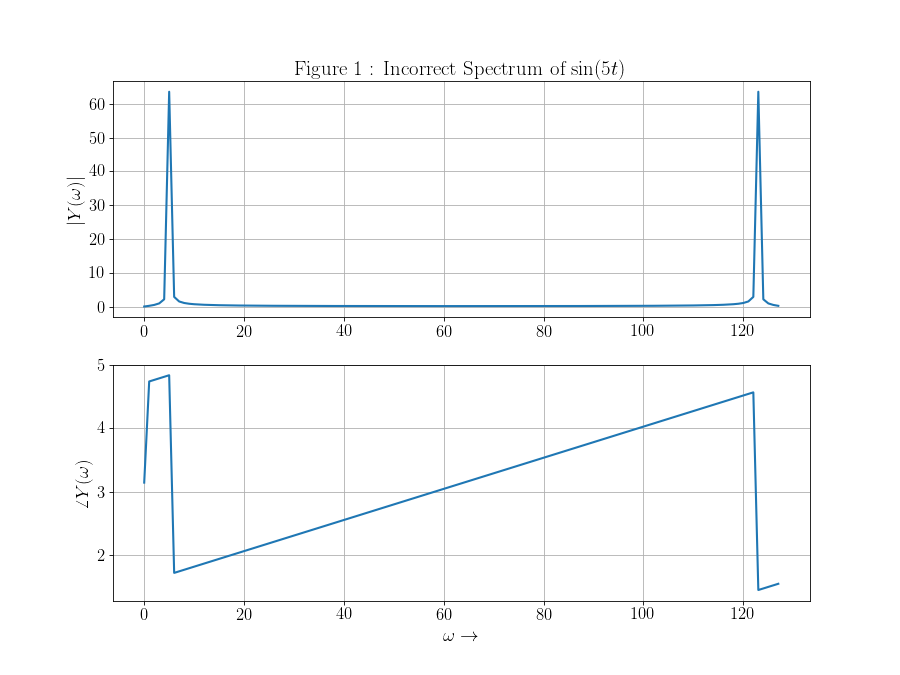
\includegraphics[scale=0.5]{./../Extras/fig9-1.png}  % Mention the image name within the curly braces. Image should be in the same folder as the tex file. 
    \caption{Incorrect Fourier spectrum plots of $sin(5t)$}
  \end{figure}
\newpage
\begin{figure}[!tbh]
  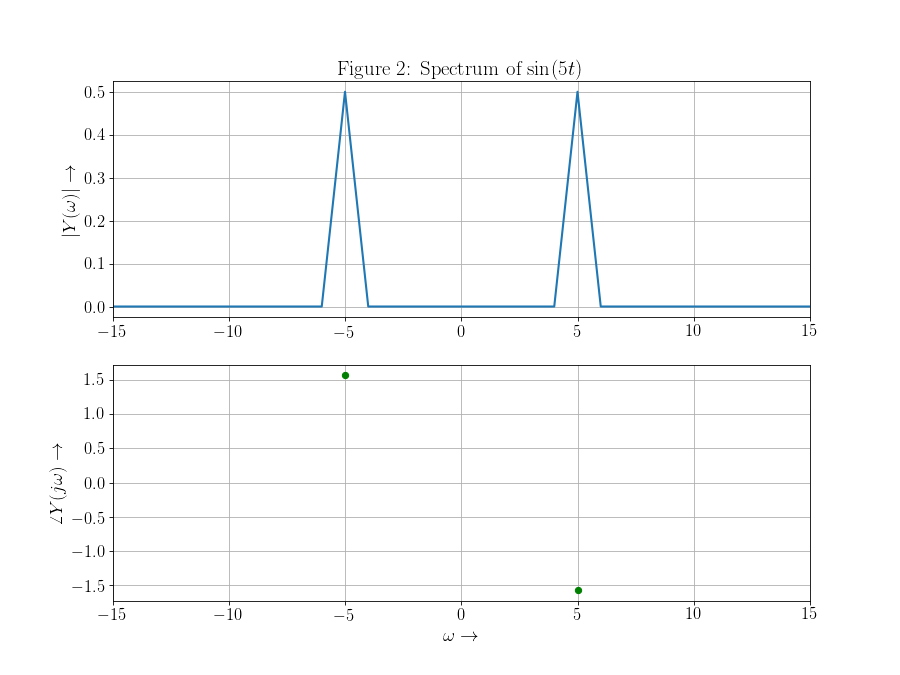
\includegraphics[scale=0.5]{./../Extras/fig9-2.png}  % Mention the image name within the curly braces. Image should be in the same folder as the tex file. 
  \caption{Correct Fourier spectrum plots of $sin(5t)$}
\end{figure}
\newpage
\subsubsection{Results and Discussion :}\label{results-and-discussion}

\begin{itemize}
\item
  The initial plot is not wrong, but is poorly labelled in x and y axes, so 
  can be generally assumed to be incorrect. The correct plot is got from using the $fftshift()$ function,
  which shifts the fft() function output between a window of interest.
  \item
  As we observe the plot frequency contents are of
  \(\omega = 5rads^{-1} ,\newline -5 rads^{-1}\)
\item
  Since everything consists of \(sin\) terms so phase is zero and
  \(\pi\) alternatively. For amplitude of the spectra we analyse the
  fourier transform of \(sin(5t)\) which is derived above.
\end{itemize}
\newpage 
\begin{figure}[!tbh]
  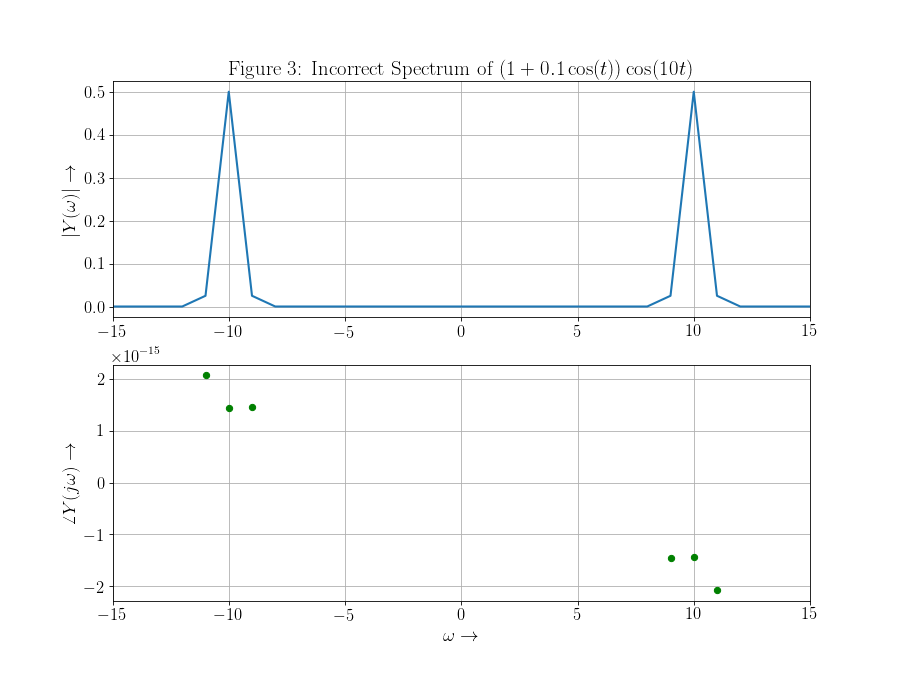
\includegraphics[scale=0.5]{./../Extras/fig9-3.png}  % Mention the image name within the curly braces. Image should be in the same folder as the tex file. 
  \caption{Incorrect Fourier spectrum plots of $\left(1+0.1\cos\left(t\right)\right)\cos\left(10t\right)$}
\end{figure}
\newpage
\begin{figure}[!tbh]
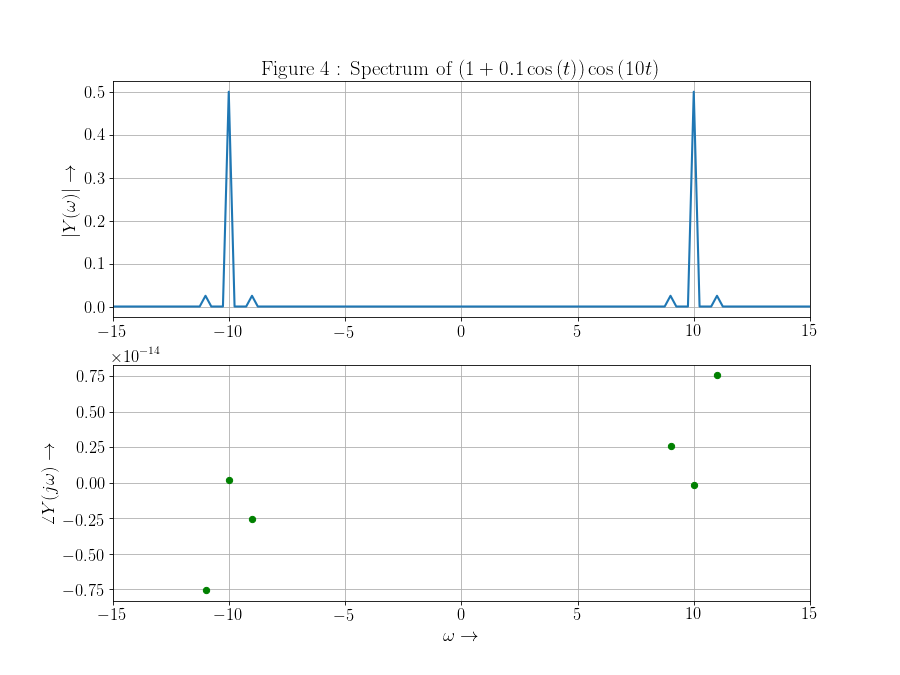
\includegraphics[scale=0.5]{./../Extras/fig9-4.png}  % Mention the image name within the curly braces. Image should be in the same folder as the tex file. 
\caption{Correct Fourier spectrum plots of $\left(1+0.1\cos\left(t\right)\right)\cos\left(10t\right)$}
\end{figure}
\newpage
\subsubsection{Results and Discussion :}\label{results-and-discussion}

\begin{itemize}
\item
  The first plot is incorrect because we did not take enough window size for the plots to be perfectly shown, thus the smaller frequency of \(2\pi\) gets
  hidden. To bring them out we must increase number of points in time domain, for the smaller frequencies to show up, whose output is shown in second plot.

\item
  As we observe the plot it has center frequencies of
  \(\omega = 10,-10\) from carrier signal and as expected we get side band frequencies at \(\omega = \pm 9 , \pm 11 \) .Since amplitude of
  the message signal is changed by a carrier signal \(\cos(10t)\) . It
  is called as amplitude modulation. And the amplitude of the side band
  frequencies are obtained from fourier transform expression.
\item
  Phase spectra is 0 since only \(\cos \) terms are present.
\end{itemize}	
\newpage
\subsection{Question 2:}\label{question-2}

\begin{itemize}

\item
  To find Discrete Fourier Transform \(DFT\) of \(\sin ^{3}(t)\) and
  \(\cos^{3}(t)\)
\item
  Plot and analyse the spectrum obtained for both the functions given
  above.
\item
  Cross validate the spectrum obtained with what is expected.
\item
  To compare the spectrum obtained for \(\sin^{3}(t)\), we use
\end{itemize}

\begin{equation}
\sin^{3}(t) = \frac{3}{4}\sin(t) - \frac{1}{4}\sin(3t)
\end{equation}

\begin{itemize}

\item
  So the fourier transform of \(\sin^{3}(t)\) using above relation is
\end{itemize}

\begin{equation}
\mathscr{F}({\sin^{3}(t)})  \to \frac{3}{8j}(\ \delta(\omega -1) - \delta(\omega+1) \ ) - \frac{1}{8j}(\ \delta(\omega -3) - \delta(\omega+3) \ )
\end{equation}

\begin{itemize}

\item
  Similarly \(\cos^{3}(t)\) is given by
\end{itemize}

\begin{equation}
\cos^{3}(t) = \frac{3}{4}\cos(t) + \frac{1}{4}\cos(3t)
\end{equation}

\begin{itemize}

\item
  So the fourier transform of \(\sin^{3}(t)\) using above relation is
\end{itemize}

\begin{equation}
\mathscr{F}({\cos^{3}(t)})  \to \frac{3}{8j}(\ \delta(\omega -1) + \delta(\omega+1) \ ) + \frac{1}{8j}(\ \delta(\omega -3) + \delta(\omega+3) \ )
\end{equation}

\begin{itemize}

\item
  So using this we compare the plots of Magnitude and phase spectrum
  obtained using \(DFT\) and analyse them.
\end{itemize}

\textit{\textbf{Code:}}
   \begin{lstlisting}
t, Y, w = findFFT(-4*pi, 4*pi, 512, f, 3)
Xlims = [-15, 15]
Ylims = []
plot_FFT(t, Y, w, 1e-4, Xlims, 
  r"Figure 5: Spectrum of $\sin ^{3}(t)$", "5")

t, Y, w = findFFT(-4*pi, 4*pi, 512, f, 4)
Xlims = [-15, 15]
plot_FFT(t, Y, w, 1e-4, Xlims, 
  r"Figure 6: Spectrum of $\cos^{3}(t)$", "6")

  \end{lstlisting}
   \newpage
   \begin{figure}[!tbh]
    \centering
    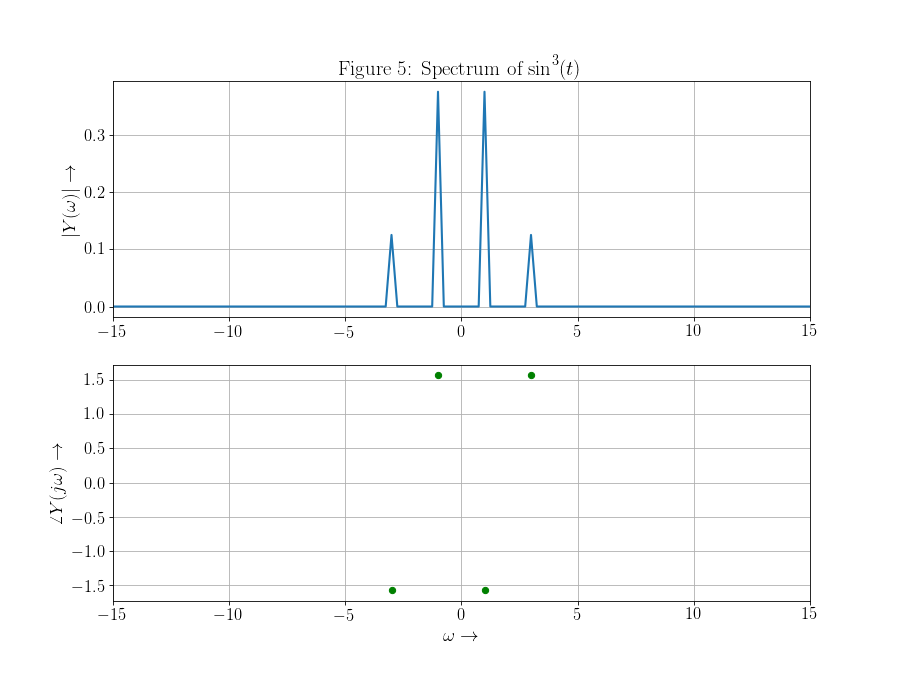
\includegraphics[scale=0.5]{./../Extras/fig9-5.png}  % Mention the image name within the curly braces. Image should be in the same folder as the tex file. 
   \caption{Spectrum of $sin^{3}(t)$}
  \end{figure}
  \newpage
  \begin{figure}[!tbh]
   \centering
   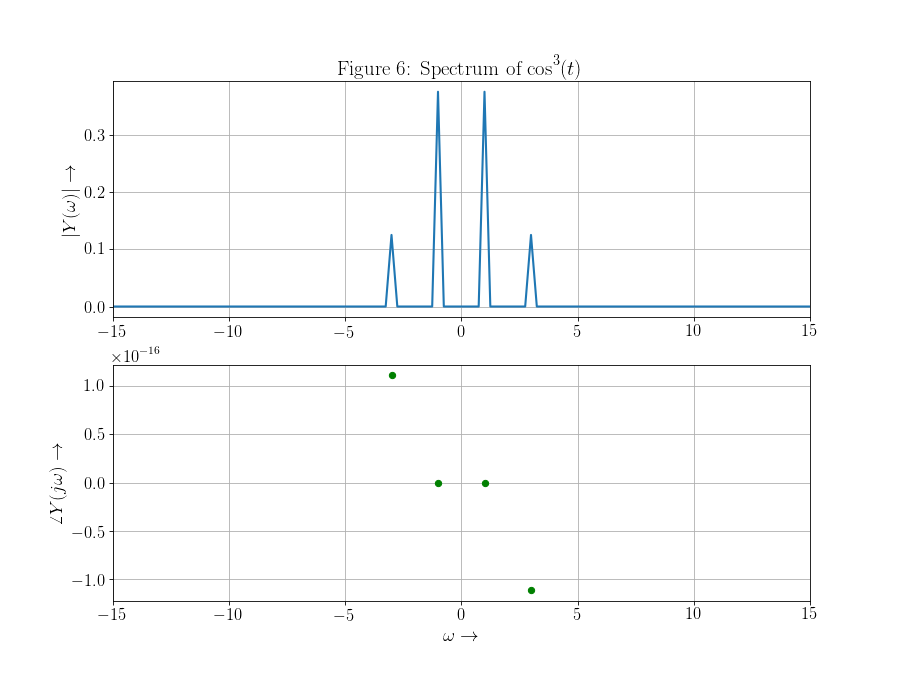
\includegraphics[scale=0.5]{./../Extras/fig9-6.png}  % Mention the image name within the curly braces. Image should be in the same folder as the tex file. 
  \caption{Spectrum of $cos^{3}(t)$}
 \end{figure}
 \newpage
 \subsubsection{Results and Discussion :}\label{results-and-discussion}

 \begin{itemize}
 
 \item
   As we observe the plot frequency contents are of
   \(\omega = 1,-1,3,-3\) and with their amplitude in 1:3 ratio
   \item
   For \(sin^{3}(t)\), since everything consists of \(\cos \) terms so phase is zero. But due
   to lack of infinite computing power they are nearly zero in the order
   of \
   \item
   For \(cos^{3}(t)\), since everything consists of \(\sin \) terms so phase is zero and
   \(\pi\) alternatively.
 \end{itemize}
 \newpage

 \subsection{Question 3:}\label{question-3}

 \begin{itemize}
 
 \item
   To generate the spectrum of \(\cos(20t +5\cos(t))\).
 \item
   Plot phase points only where the magnitude is significant
   (\(\ > 10^{-3}\)).
 \item
   Analyse the spectrums obtained.
 \end{itemize}
\textit{\textbf{Code:}}
\begin{lstlisting}
t, Y, w = findFFT(-4*pi, 4*pi, 512, f, 5)
Xlims = [-40, 40]
plot_FFT(t, Y, w, 1e-3, Xlims, r"Figure 7: Spectrum of $\cos(20t+5\cos(t))$", "7")
  
\end{lstlisting}
\newpage
\begin{figure}[!tbh]
  \centering
  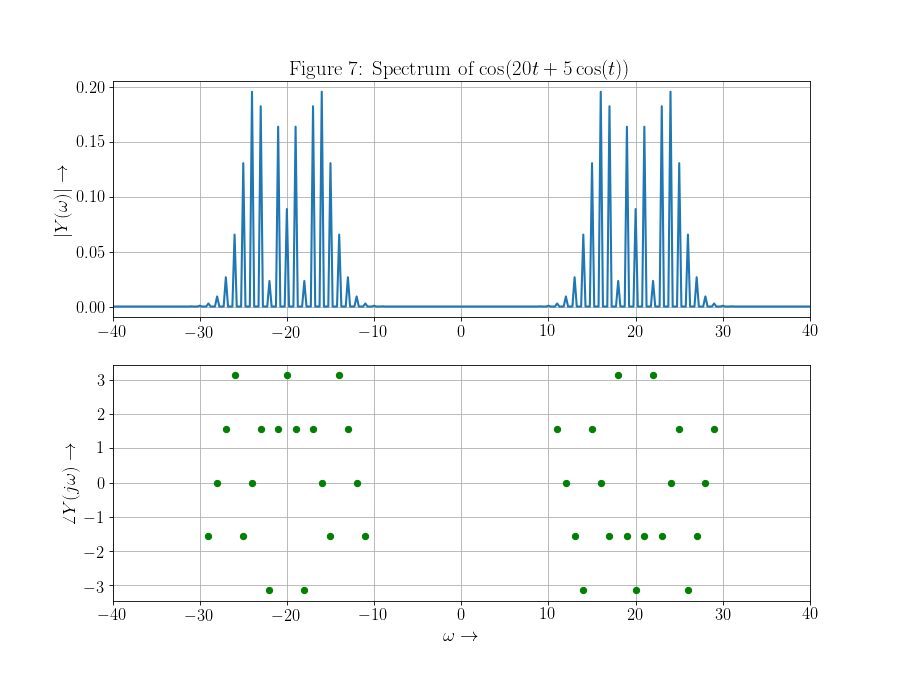
\includegraphics[scale=0.5]{./../Extras/fig9-7.png}  % Mention the image name within the curly braces. Image should be in the same folder as the tex file.  
  \caption{Spectrum of $\cos(20t+5\cos(t))$}
\end{figure}

\newpage
\subsubsection{Results and Discussion :}\label{results-and-discussion}

\begin{itemize}

\item
  As we observe the plot that its a Phase modulation since phase of the
  signal is varying proportional to amplitude of the message signal
  being \(\omega = 20\) and infinite side band frequencies which are
  produced by \(5\cos t\). since \(\cos(t)\) is infinitely long signal.
  But the strength of the side band frequencies decays or very small
  which are away from center frequency or carrier frequency component as
  we observe from the plot.
\item
  Phase spectra is a mix of different phases from \([-\pi,\pi]\) because
  of phase modulation, i.e since the phase is changed continuously wrt
  time, the carrier signal can represent either a \(sine\) or \(cosine\)
  depending on the phase contribution from \(cos(t)\).
\end{itemize}

\subsection{Question 4:}\label{question-4}

\begin{itemize}

\item
  To generate the spectrum of the Gaussian \(e^{-\frac{t^{2}}{ 2}}\)
  which is not \(bandlimited\) in frequency and aperiodic in time domain
  find Fourier transform of it using DFT and to recover the analog
  fourier transform from it.
\end{itemize}

\begin{equation}
 \mathscr{F} ( \ e^{-\frac{t^{2}}{2}} \ ) \to \frac{1}{\sqrt 2\pi} e^{\frac{\ - \omega ^{2}}{2}}
\end{equation}

\begin{itemize}

\item
  To find the normalising constant for DFT obtained we use following
  steps to derive it :
\item
  window the signal \(e^{-\frac{t^{2}}{2}}\) by rectangular function
  with gain 1 and window\_size 'T' which is equivalent to convolving
  with \(Tsinc(\omega T)\) in frequency domain. So As T is very large
  the \(sinc(\omega T) \) shrinks , we can approximate that as
  \(\delta(\omega)\) . So convolving with that we get same thing.
\item
  Windowing done because finite computing power and so we cant represent
  infinetly wide signal .
\item
  Now we sample the signal with sampling rate N,which is equivalent to
  convolving impulse train in frequency domain
\item
  And finally for DFT we create periodic copies of the windowed sampled
  signal and make it periodic and then take one period of its Fourier
  transform i.e is DFT of gaussian.
\item
  Following these steps we get normalising factor of
  \textbf{Window\_size/(\(2 \pi \ \)Sampling\_rate)}
\end{itemize}

\begin{equation}
exp({-\frac{t^2}{2}}) \longleftrightarrow \frac{1}{\sqrt{2\pi}}exp({-\frac{\omega^2}{2}})
\end{equation}

\begin{equation}
rect(\frac{t}{\tau}) =
\begin{cases}
1\  for\ |t| < \tau \\
0\ otherwise
\end{cases}
\end{equation}

\begin{itemize}

\item
  For windowing the signal, we will multiply with the rectangular
  function,
\end{itemize}

\begin{equation}
y(t) = gaussian(t) \times rect(\frac{t}{\tau})
\end{equation}

\begin{itemize}

\item
  In fourier domain, its convolution (since multiplication is
  convolution in fourier domain)
\end{itemize}

\begin{equation}
Y(\omega) = \frac{1}{2\pi}(\frac{1}{\sqrt{(2\pi)}}e^{-\omega^2/2} * \frac{sin(\tau \omega)}{\omega})
\end{equation}

\begin{equation}
\lim_{\tau \to\infty} Y(\omega) = \frac{\tau}{2\pi}(\frac{1}{\sqrt{(2\pi)}}e^{-\omega^2/2} * \delta(\omega))
\end{equation}

\begin{equation}
\lim_{\tau \to\infty} Y(\omega) = \frac{\tau}{2\pi}(\frac{1}{\sqrt{(2\pi)}}e^{-\omega^2/2})
\end{equation}

\begin{itemize}

\item
  Now, sampling this signal with a period of \(\frac{2\pi}{T_s}\), we
  will get (multiplication by an impulse train in fourier domain),
\end{itemize}

\begin{equation}
Y_{sampled} = \frac{\tau}{2\pi T_s}\frac{1}{\sqrt{(2\pi)}}e^{-\omega^2/2} \sum_{k = -\infty}^{\infty}\delta(\omega - \frac{k2\pi}{T_s})
\end{equation}

\begin{itemize}

\item
  Solving it further we get the multiplication factor to be,
\end{itemize}

\begin{equation}
const = \frac{\tau}{T_s 2\pi}
\end{equation}

\begin{itemize}

\item
  To find the Discrete Fourier transform equivalent for Continous
  Fourier transform of Gaussian function by finding absolute error
  between the DFT obtained using the normalising factor obtained with
  exact Fourier transform and find the parameters such as Window\_size
  and sampling rate by minimising the error obtained with tolerance of
  \(10^{-15}\)
\item
  To generate the spectrum
\item
  Plot phase points only where the magnitude is significant
  (\(\ > 10^{-2}\)).
\item
  Analyse the spectrums obtained.
\end{itemize}

\textit{\textbf{Code:}}
   \begin{lstlisting}
window_size = 2*pi
sampling_rate = 128
# tolerance for error
tol = 1e-15

# normalisation factor derived
norm_factor = (window_size)/(2*pi*(sampling_rate))


'''
For loop to minimize the error by increasing 
both window_size and sampling rate as we made assumption that
when Window_size is large the sinc(w) acts like impulse, so we
increase window_size, similarly sampling rate increased to 
overcome aliasing problems
'''

for i in range(1, 10):

    t, Y, w = findFFT(-window_size/2, window_size/2,
                      sampling_rate, f, 6, norm_factor)

    # actual Y
    actual_Y = (1/sqrt(2*pi))*exp(-pow(w, 2)/2)
    error = (np.mean(np.abs(np.abs(Y)-actual_Y)))
    print("Absolute error at Iteration - %g is : %g" % ((i, error)))

    if(error < tol):
        print("\nAccuracy of the DFT is: %g and Iterations took: %g" %
              ((error, i)))
        print("Best Window_size: %g , Sampling_rate: %g" %
              ((window_size, sampling_rate)))
        break
    else:
        window_size = window_size*2
        sampling_rate = (sampling_rate)*2
        norm_factor = (window_size)/(2*pi*(sampling_rate))


Xlims = [-10, 10]
plot_FFT(t, Y, w, 1e-2, Xlims,
         r"Figure 8: Spectrum of $e^{-\frac{t^{2}}{ 2}}$", "8")

# Plotting actual DFT of Gaussian
plot(w, abs(actual_Y),
     label=r"$\frac{1}{\sqrt{2}\pi} e^{\frac{\ - \omega ^{2}}{2}}$")
title("Exact Fourier Transform of Gaussian")
xlim([-10, 10])
ylabel(r"$Y(\omega) \to$")
xlabel(r"$\omega \to$")
grid()
legend()
show()

   \end{lstlisting}
   \newpage
   \begin{figure}[!tbh]
     \centering
     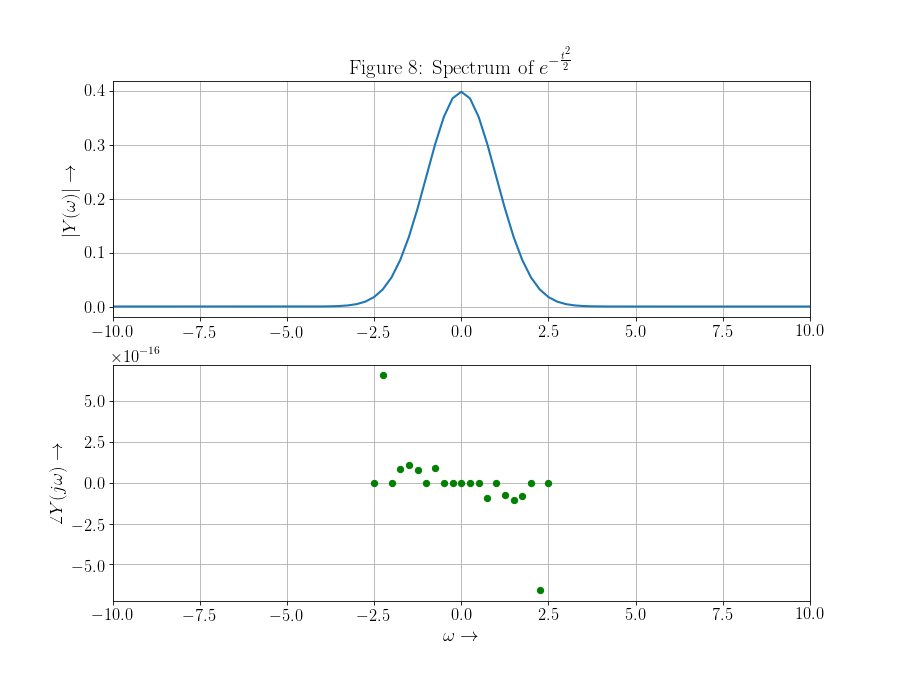
\includegraphics[scale=0.4]{./../Extras/fig9-8.png}  % Mention the image name within the curly braces. Image should be in the same folder as the tex file.  
     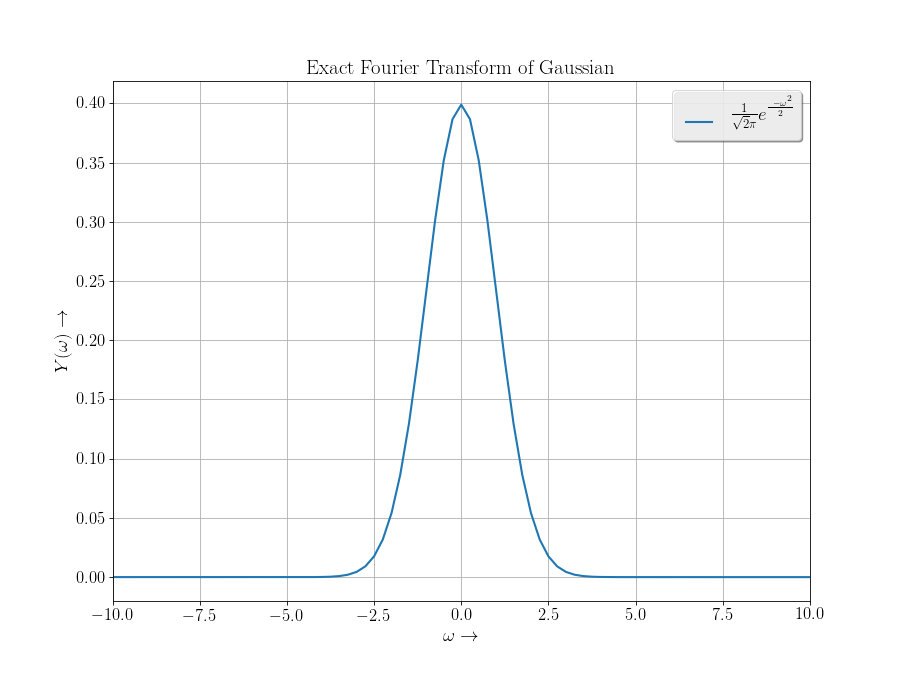
\includegraphics[scale=0.4]{./../Extras/fig9-9.png}  % Mention the image name within the curly braces. Image should be in the same folder as the tex file.  
     \caption{Spectrum of $\cos(20t+5\cos(t))$}
   \end{figure}
   
   \newpage
   
		
   \subsubsection{Results and Discussion :}\label{results-and-discussion}

   \begin{itemize}
   \item
Absolute error at Iteration - 1 is : 5.20042e-05\newline
Absolute error at Iteration - 2 is : 2.07579e-11\newline
Absolute error at Iteration - 3 is : 4.14035e-17\newline

Accuracy of the DFT is: 4.14035e-17 and Iterations took: 3 \newline
Best Window\_size: 25.1327 , Sampling\_rate: 512

   \item
     As we observe the magnitude spectrum of \(e^{-\frac{t^{2}}{ 2}}\) we
     see that it almost coincides with exact Fourier Transform plotted
     below with accuracy of \(4.14035e^{-17}\)
   \item
     To find the correct Window size and sampling rate,For loop is used to
     minimize the error by increasing both window\_size and sampling rate
     as we made assumption that when Window\_size is large the sinc(wT)
     acts like impulse \(\delta(\omega)\)
   \item
     so we increase window\_size, similarly sampling rate is increased to
     overcome aliasing problems when sampling the signal in time domain.
   \item
     Similarly we observe the phase plot ,\(\angle(Y(\omega) \approx 0\) in
     the order of \(10^{-15}\) if we magnify and observe
   \end{itemize}
   
     
   
     
       
       \subsection{Conclusion :}\label{conclusion}
   
   \begin{itemize}
   
   \item
     Hence we analysed the how to find DFT for various types of signals and
     how to estimate normalising factors for Gaussian functions and hence
     recover the analog Fourier transform using DFT ,also to find
     parameters like window\_size and sampling rate by minimizing the error
     with tolerance upto \(10^{-15}!!\)
   \item
     We used fast Fourier transform method to compute DFT as it improves
     the computation time from
     \(\mathcal{O} n^2 \to \mathcal{O} n\log_2(n)\).
   \item
     FFT works well for signals with samples in \(2^{k}\) , as it divides
     the samples into even and odd and goes dividing further to compute the
     DFT.
   \item
     That's why we use no of samples in the problems above taken as powers
     of \(2\).
   \end{itemize}
   
     
	
		
	
		
			
		

      
\end{document}